%% TODO: Add a small paragraph to tell what this chapter is about
This chapter presents a thorough exposition of the architecture and implementation details of the Test Genie system. Throughout the development process, considerable attention was devoted to creating a modular and extensible architecture that could accommodate future enhancements while maintaining robust functionality. The system architecture comprises three principal modules, each fulfilling distinct yet interdependent functions:

\begin{itemize}
    \item[-] \textbf{Project Manager}: This foundational module orchestrates repository management operations, handling Git interactions, local file system management, and framework-specific command-line interface executions. During its development, particular consideration was given to ensuring framework agnosticism through an abstract design pattern.
    
    \item[-] \textbf{Business Logic Analyzer (BLA)}: Serving as the analytical core, this module ingests source files from the Project Manager and decomposes them into semantically meaningful blocks through a series of sophisticated parsing algorithms. Each block undergoes analysis to determine its functionality and testing requirements, subsequently generating test plans that are persisted in the database infrastructure. The development of these analytical algorithms represented one of the most challenging aspects of the implementation.
    
    \item[-] \textbf{Test Generator}: This module transforms analytical insights from the BLA into executable test cases through a carefully designed generation process. The tests are integrated directly into the project's structure, enabling immediate validation. Significant effort was invested in ensuring the generator could handle various edge cases and framework-specific testing requirements.
\end{itemize}

The system also incorporates a supplementary \textbf{DBMS} module for persistent storage operations, which, while not a primary focus of this chapter, plays an essential role in maintaining system state across execution cycles.

%% TODO: Make sure to use \textbf or \textit for highlighting keywords, and \cite{} to cite the corresponding quotations

\section{Project Manager module}

The \textbf{ProjectManager} module constitutes the foundation upon which the Test Genie system operates, providing essential interfaces for repository management and framework-specific operations. During the design phase, I deliberated extensively on the appropriate architectural pattern to ensure both flexibility and robustness. After evaluating several alternatives, I settled on an abstract base class design that enables framework-specific extensions through inheritance.

The central component of this module, the \textit{Project} class, encapsulates common repository management functionality while deferring framework-specific operations to specialized subclasses. This design decision was motivated by the observation that while Git operations remain relatively consistent across projects, testing frameworks exhibit significant variability in their setup, execution, and validation requirements. By establishing a clear separation of concerns between generic and framework-specific operations, the system achieves remarkable extensibility without sacrificing cohesion.

The subclass architecture exemplifies the Template Method design pattern, wherein the base class defines the operational structure while concrete implementations furnish the specialized behavior required by different frameworks. This approach proved particularly valuable when implementing the Flutter-specific functionality, as it permitted focused development of framework-specific features without modifying the underlying repository management infrastructure.

\subsection{Module prequisites}

After careful consideration of deployment options, I determined that framework SDKs should be installed within dedicated directories (\textit{./SDKs}) rather than relying on system-wide installations. This architectural decision, while introducing initial configuration complexity, offers several substantial advantages:

\begin{itemize}
    \item[-] It ensures version consistency across different deployment environments, mitigating the risk of compatibility issues
    \item[-] It facilitates containerization by encapsulating all dependencies within the application directory
    \item[-] It prevents conflicts with existing installations, enhancing system stability
    \item[-] It simplifies the process of supporting additional frameworks, as each can maintain its isolated environment
\end{itemize}

To maintain consistency across framework implementations, I established a contract requiring subclasses to implement the following methods:
    \begin{itemize}
        \item[-] \textbf{create\_test}: Responsible for generating appropriately structured test files in framework-specific locations, adhering to established naming conventions and directory structures
        \item[-] \textbf{get\_test\_content}: Facilitates retrieval of test content, ensuring proper formatting and structural integrity
        \item[-] \textbf{run\_test}: Executes tests using framework-native commands, capturing output and error messages for subsequent analysis
        \item[-] \textbf{validate}: Conducts comprehensive validation across all test files, providing consolidated results to assess overall test quality
        \item[-] \textbf{getListSourceFiles}: Perhaps the most critical method, as it determines the entry points and traversal order for source code analysis, significantly influencing the effectiveness of subsequent analytical processes
    \end{itemize}


\subsection{Flutter class}

The \textbf{Flutter} class represents the concrete implementation of the abstract \textbf{Project} interface for Flutter framework projects. Developing this class presented several unique challenges, particularly related to the dynamic nature of Flutter's toolchain and its evolving command-line interface. Through empirical testing and refinement, I established a robust set of operations that reliably manage Flutter-specific aspects of project analysis and test execution.

The implementation encompasses several key operational areas:
\begin{itemize}
    \item[-] \textbf{Flutter SDK Management}: The \texttt{\_runFlutterCLI} and \texttt{\_checkSDK} methods required careful implementation to handle various environment configurations and potential SDK installation issues. Particular attention was given to error handling to provide meaningful feedback when SDK anomalies occur.
    
    \item[-] \textbf{Dependency Management}: Through extensive experimentation, I determined that the \texttt{\_flutterPubGet} and \texttt{\_addTestDependency} methods needed special handling to manage Flutter's package ecosystem effectively. These methods ensure that all required testing dependencies are properly installed without disrupting existing project configurations.
    
    \item[-] \textbf{Test File Operations}: The \texttt{create\_test} and \texttt{get\_test\_content} implementations adhere to Flutter's convention of housing test files in a dedicated \texttt{test} directory, with proper handling of existing files to prevent accidental overwrites.
    
    \item[-] \textbf{Test Execution}: The \texttt{run\_test} method employs Flutter's built-in test runner with appropriate configuration parameters to ensure reliable test execution. Significant effort was devoted to capturing and parsing test output to distinguish between test failures and execution errors.
    
    \item[-] \textbf{Source File Enumeration}: The \texttt{getListSourceFiles} implementation required careful consideration of Flutter's directory structure conventions. It ensures that the application entry point (\texttt{main.dart}) receives priority treatment, as this file typically contains critical structural information about the application.
\end{itemize}

This implementation represents a balance between adhering to Flutter's conventions and maintaining compatibility with the broader Test Genie architecture. The resulting class provides a seamless integration point for Flutter projects within the system.

\section{Business Logic Analyzer module}

The \textbf{Business Logic Analyzer} module constitutes the intellectual core of the Test Genie system. Its development presented some of the most intricate challenges encountered during the implementation phase, requiring a sophisticated approach to code comprehension and semantic analysis. After evaluating multiple parsing strategies, including the use of formal Abstract Syntax Tree (AST) parsers, I ultimately developed a custom analysis approach that balances performance requirements with analytical depth.

The module's primary function—decomposing source code into meaningful blocks and extracting their semantic relationships—demanded careful consideration of programming language structures and idioms. Rather than relying solely on syntactic parsing, which often fails to capture semantic nuances, I developed a multi-layered analysis strategy that combines structural recognition with heuristic assessment of code relationships.

At the module's core lies the \textbf{DependencyDiagram} class, which orchestrates the analysis process and maintains the resulting structural representation. This class serves as a critical bridge between raw source code and the AI-powered prediction system, transforming syntactic structures into semantically meaningful units amenable to intelligent analysis.

\subsection{DependencyDiagram class}

The \textbf{DependencyDiagram} class emerged through several iterations of design refinement. Initially conceived as a simple graph structure, it evolved into a sophisticated connector between framework-specific analysis strategies and AI-powered prediction capabilities. The class maintains two fundamental collections: blocks (representing functional units) and connections (representing relationships between those units).

One of the most significant design decisions involved the method of diagram generation. After experimenting with various approaches, I implemented the \textbf{\_generateDiagram} method to dynamically select and apply the appropriate analysis strategy based on the project's framework. This approach ensures that the system can accommodate framework-specific idiosyncrasies without sacrificing analytical consistency.

The integration with the \textbf{AI\_Agent} component required careful consideration of interface design and data flow. The \textbf{\_getPredictions} method iterates through the identified blocks, submitting each to the AI agent for analysis and prediction generation. To optimize this process, I implemented rate limiting and caching mechanisms to balance analytical thoroughness with performance constraints.

Through numerous refinements and testing cycles, the \textbf{DependencyDiagram} class evolved into a robust foundation for the system's analytical capabilities, effectively bridging the gap between static code structures and dynamic semantic understanding.

\subsubsection{Diagram objects}

The representation of code structures required a carefully designed object model. After evaluating alternatives, I developed a system of interrelated classes that effectively capture the hierarchical and relational aspects of software projects:

\begin{itemize}
    \item[-] \textbf{Block class}: This class emerged as the fundamental unit of representation after several design iterations. Initial implementations focused solely on content storage, but experience revealed the need for additional capabilities such as comment filtering (via the \textbf{getContentNoComment} method) and metadata management. Each block encapsulates:
    \begin{itemize}
        \item[-] \textit{name}: An identifier that uniquely represents the block within its context
        \item[-] \textit{content}: The actual source code, preserved in its original form for reference and analysis
        \item[-] \textit{type}: A classification determined by the BlockType enumeration, indicating the block's role within the codebase
        \item[-] \textit{prediction}: An AI-generated assessment of the block's purpose and behavior, integrated after analysis
    \end{itemize}

    \item[-] \textbf{BlockType class}: This enumeration evolved from simple string constants to a structured class that supports both programmatic operation and database persistence. The comprehensive set of types emerged through detailed analysis of Flutter codebases, ensuring coverage of all relevant structural elements.

    \item[-] \textbf{Connection class}: This class represents the relationships between blocks, capturing the directional nature of software dependencies. Each connection maintains references to both the source and destination blocks, along with a classification of the relationship type.

    \item[-] \textbf{ConnectionType class}: After studying common relationships in Flutter applications, I developed this enumeration to represent the variety of connections between code elements, from inheritance relationships to method invocations.
\end{itemize}

The development of these classes involved numerous refinements based on empirical testing with actual Flutter projects, ensuring that the object model adequately represents the complexity and nuance of real-world codebases.

\subsubsection{FlutterAnalyzeStrategy Algorithm}

The \textbf{FlutterAnalyzeStrategy} function represents one of the most technically challenging aspects of the implementation. Through extensive experimentation with Flutter projects of varying complexity, I developed a three-phase analysis approach that progressively builds a comprehensive understanding of the codebase:

\begin{itemize}
    \item[-] \textbf{Initialization Phase:}
    \begin{itemize}
        \item The function begins by retrieving source files through the \textbf{getListSourceFiles} method, prioritizing the entry point (typically \texttt{main.dart}) to establish the analytical foundation.
        \item Initial testing revealed the importance of preserving the original file structure in the analysis, leading to the creation of file-level blocks that serve as containers for more granular elements.
    \end{itemize}

    \item[-] \textbf{Import Analysis Phase (ImportAnalyzer):}
    \begin{itemize}
        \item Early prototype testing demonstrated that understanding import relationships provides crucial context for subsequent analysis. The \textbf{ImportAnalyzer} algorithm scans for import statements and establishes connections between files.
        \item A particular challenge involved resolving relative imports correctly, necessitating sophisticated path normalization routines to handle various import syntaxes consistently.
    \end{itemize}

    \item[-] \textbf{Containment Analysis Phase (ContainAnalyzer):}
    \begin{itemize}
        \item This phase represents the most sophisticated component of the analysis, employing a state machine approach to track brackets, indentation, and contextual keywords.
        \item Initial implementations using simple regex patterns proved insufficient, leading to the development of a contextual parser that maintains awareness of nested structures and their hierarchical relationships.
        \item The algorithm identifies classes, functions, methods, and attributes, creating appropriate blocks and connections to represent their containment relationships.
    \end{itemize}

    \item[-] \textbf{Call Analysis Phase (CallAnalyzer):}
    \begin{itemize}
        \item The final analytical phase identifies calling relationships between functions and methods, which proved particularly challenging due to the syntactic flexibility of Dart.
        \item After several iterations, I developed a hybrid approach combining structural context with pattern matching to identify method invocations across class and file boundaries.
        \item Performance optimization was essential for this phase, as naive implementation would result in quadratic complexity. The final algorithm employs type filtering and early termination to maintain practical performance characteristics.
    \end{itemize}
\end{itemize}

This multi-phase approach evolved through continuous refinement and testing against increasingly complex Flutter projects. The resulting algorithm successfully balances analytical depth with computational efficiency, producing detailed and accurate dependency diagrams that serve as the foundation for subsequent test generation.

\subsection{AI\_Agent class}

The \textbf{AI\_Agent} class represents the integration point between traditional code analysis and advanced artificial intelligence capabilities. Its development required careful consideration of both technical constraints and pedagogical principles to ensure effective analysis of code blocks. By leveraging the \textit{Langchain framework} ~\cite{langchain}, I constructed a sophisticated analytical pipeline that combines retrieval-augmented generation with domain-specific prompting.

\subsubsection{Initialization Flow}

The initialization process for the \textbf{AI\_Agent} class underwent several iterations before reaching its current form. Early implementations suffered from brittle environment configuration and resource management issues, leading to the development of a more robust initialization sequence:

\begin{itemize}
    \item[-] \textbf{Environment Setup:}
    \begin{itemize}
        \item Initial testing revealed the importance of graceful handling of configuration issues. The current implementation employs careful validation of environment variables with meaningful error messages when critical values are missing.
        \item The most critical configuration parameters include API endpoints, model selection, and embedding specifications, which significantly impact analysis quality and performance.
    \end{itemize}

    \item[-] \textbf{Model and Embedding Initialization:}
    \begin{itemize}
        \item Selection of appropriate models for both generation and embedding tasks required extensive experimentation to balance quality with performance constraints.
        \item Special attention was given to embedding configuration, as early testing revealed compatibility issues with certain vector database implementations, necessitating parameter adjustments.
    \end{itemize}

    \item[-] \textbf{Vector Store Creation:}
    \begin{itemize}
        \item Initial implementations recreated vector stores on each initialization, leading to significant startup delays. The current approach employs persistent storage with intelligent reuse to optimize initialization time.
        \item Document selection proved critical for effective retrieval-augmented generation. After testing various combinations, I determined that Flutter-specific documentation provides the most relevant context for code analysis.
        \item Document chunking strategies underwent several refinements to optimize retrieval accuracy, with sentence-based transformers ultimately providing the best balance of semantic coherence and granularity.
    \end{itemize}

    \item[-] \textbf{Retriever Configuration:}
    \begin{itemize}
        \item Early testing with simple similarity-based retrieval yielded inconsistent results, leading to the implementation of threshold-based retrieval with carefully tuned parameters.
        \item Extensive experimentation with similarity thresholds revealed that a value of 0.4 provides the optimal balance between recall and precision for Flutter code analysis.
    \end{itemize}

    \item[-] \textbf{Agent Initialization:}
    \begin{itemize}
        \item The agent architecture evolved from simple query-response patterns to a more sophisticated history-aware system capable of maintaining context across analysis operations.
        \item Prompt engineering represented a significant challenge, requiring numerous iterations to develop instructions that reliably produce structured and useful analysis outputs.
    \end{itemize}
\end{itemize}

\subsubsection{generate\_BLA\_prediction Function}

The \textbf{generate\_BLA\_prediction} function embodies the core analytical capability of the system. Through careful design and iterative refinement, I developed a two-stage analysis process that combines exploratory analysis with structured output generation:

1. The first stage employs the agent executor to perform open-ended analysis of the provided code snippet. Early implementations produced verbose but unstructured outputs, prompting the development of agent-specific prompting strategies to focus the analysis on relevant aspects of the code's functionality.

2. The second stage applies structured prompting to organize the initial analysis into a consistent format suitable for test generation. Extensive prompt engineering was required to consistently produce outputs with well-defined sections covering:
   - Concise functional explanations that capture the essence of the code's purpose
   - Testability assessments that identify appropriate testing approaches and potential challenges
   - Detailed testing scenarios with specific inputs and expected outputs

A particularly challenging aspect of implementation involved ensuring consistent formatting of testing scenarios. Initial attempts often produced scenarios with insufficient specificity, leading to the development of explicit formatting instructions with examples. The final implementation consistently generates detailed scenarios with descriptive test names, clear functionality descriptions, specific input values, and well-defined expected outcomes.

The function's effectiveness stems from its combination of retrieval-augmented generation, which incorporates domain-specific knowledge about Flutter and testing practices, with carefully structured prompting that ensures consistent and useful outputs. This approach significantly enhances the quality of analysis compared to simple prompt-completion models, as evidenced by comparative testing with alternative approaches.

\subsection{Test Generator Module}

The \textbf{Test Generator} module represents the culmination of the Test Genie system's analytical capabilities, transforming abstract predictions into concrete, executable test cases. Developing this module presented unique challenges at the intersection of template generation, context management, and error correction. Through iterative refinement and extensive testing with real-world Flutter projects, I developed a robust generation and validation pipeline that produces high-quality test cases.

\subsubsection{Initialization Flow}

The initialization process for the \textbf{Test\_Generator} class builds upon the architectural patterns established in the \textbf{AI\_Agent} class, with specific adaptations for test generation requirements:

\begin{itemize}
    \item[-] \textbf{Environment Setup:} After examining various configuration management approaches, I selected a dotenv-based configuration with fallback mechanisms to ensure robustness across deployment environments. Critical parameters include model selection and API endpoints specific to test generation tasks.

    \item[-] \textbf{Model and Embedding Initialization:} Test generation presents different challenges than code analysis, requiring models with strong code generation capabilities. Testing with various models led to the selection of specific configurations optimized for generating valid Dart test code.

    \item[-] \textbf{Vector Store Management:} Drawing on insights from the \textbf{AI\_Agent} implementation, I developed an optimized approach to vector store management that retains the benefits of retrieval-augmented generation while minimizing initialization overhead. Document selection focused on Flutter testing documentation to ensure generated tests follow framework-specific best practices.

    \item[-] \textbf{Error Handling Infrastructure:} A distinguishing feature of this module is its sophisticated error handling system, developed after observing common failure patterns in test generation:
    \begin{itemize}
        \item An error cache with intelligent lookup mechanisms prevents redundant correction attempts for similar errors
        \item A tracking system for attempted fixes avoids infinite correction loops
        \item A configurable retry limit system balances correction thoroughness with execution efficiency
    \end{itemize}
\end{itemize}

These initialization mechanisms establish a foundation for reliable test generation with built-in resilience against common failure modes.

\subsubsection{Test Generation and Validation Flow}

The test generation process, orchestrated by the \textbf{generateTest} function in the \texttt{main.py} file, represents one of the most intricate workflows in the system. Its development required careful consideration of data flow, error handling, and validation logic to create a robust end-to-end process:

1. The process begins with parameter validation and resource initialization, establishing the project context through the \textbf{DBMS} interface. Early implementations revealed the importance of thorough parameter validation to prevent cascading errors later in the process.

2. Test case generation is performed by the \textbf{generate\_test\_case} method, which combines several critical pieces of information:
   - Package information for import statement generation
   - Code location for proper path references
   - Function signatures for accurate test targeting
   - Behavioral predictions to guide test scenario implementation

3. The generated test is saved to the project structure using the \textbf{Project} class's \texttt{create\_test} method. Initial implementations encountered path resolution issues, leading to the development of more robust path handling routines.

4. Validation is performed by executing the test using the \texttt{run\_test} method. This critical step distinguishes Test Genie from many other generation approaches by ensuring that tests are not merely syntactically correct but also executable.

5. Error correction, when necessary, employs the \textbf{fix\_generated\_code} method to iteratively refine failed tests. This process represents one of the most sophisticated aspects of the system, combining error analysis, context-aware correction, and validation in a feedback loop that continues until either success is achieved or the retry limit is reached.

Through extensive testing with diverse Flutter components, this workflow has proven highly effective at producing valid, executable tests across a range of code structures and complexities.

\subsubsection{Integration with the Test Genie System}

The integration of the test generator with the broader Test Genie system presented architectural challenges related to data flow and component coupling. Rather than adopting a tightly coupled approach, I designed an integration pattern that maintains component independence while ensuring effective collaboration:

1. The \textbf{DBMS} system serves as a central coordination point, providing access to both structural information from the Business Logic Analyzer and persistence capabilities for generated tests.

2. The test generation process leverages predictions stored in the database, creating a clean separation between analysis and generation phases while maintaining conceptual continuity.

3. The iterative correction process demonstrates the system's self-healing capabilities, with each correction attempt incorporating feedback from previous execution results to improve subsequent attempts.

This integration approach ensures that each component can evolve independently while maintaining system cohesion, facilitating both maintenance and future enhancement of the Test Genie system.

\section{Other implementations}
Beyond the core analytical and generative components, the Test Genie system incorporates several supporting modules that enhance its functionality and usability. These components, while less conceptually complex than the core modules, play essential roles in creating a cohesive and effective system:

\begin{itemize}
    \item [-] \textbf{API request handler}: Implementation of this component involved careful consideration of request validation, error handling, and response formatting. I selected the Flask framework for its minimal overhead and straightforward routing capabilities, constructing a RESTful API that exposes the system's core functionality through well-defined endpoints.
    
    \item [-] \textbf{DBMS}: Database management presented challenges related to schema design, query optimization, and transaction management. After evaluating several options, I implemented a MySQL-based persistence layer with a custom object-relational mapping approach tailored to the specific needs of the system.
    
    \item [-] \textbf{Frontend}: User interface development focused on creating an intuitive visualization and interaction system for the dependency diagram. Implementing this interface using React required careful attention to component design, state management, and performance optimization to ensure responsiveness even with complex project structures.
\end{itemize}

\subsection{DBMS module}

The database management subsystem provides persistent storage and retrieval capabilities for project metadata, blocks, and connections. Its design evolved through several iterations as the storage requirements became more clearly defined:

\subsubsection{DBMS Class}

The \textbf{DBMS} class provides the primary interface for database operations, abstracting the complexity of SQL queries and connection management. Its development involved careful consideration of initialization sequences, query execution patterns, and error handling:

1. The initialization flow employs a progressive approach, first checking database existence and initialization status before performing schema creation or updates as necessary.

2. Project management functions handle the insertion of new projects and the verification of existing ones, with special attention to handling the complex relationships between projects, blocks, and connections.

3. Data retrieval operations include specialized methods for accessing block content, predictions, and relationship information, with query optimization to ensure efficient retrieval even for large projects.

4. String handling required particular attention due to the presence of special characters in source code, leading to the implementation of the \texttt{\_handldApostropheString} method to ensure reliable storage and retrieval of code content.

This centralized approach to database management ensures consistency across the system while providing a flexible interface for component-specific storage needs.

\subsubsection{Table Class}

The \textbf{Table} class represents an innovative approach to database table management, providing dynamic SQL generation capabilities that enhance both code maintainability and query consistency. Its development involved careful consideration of SQL syntax, parameter handling, and abstraction principles:

1. Table creation operations employ parameterized column definitions, allowing for flexible schema definition while maintaining syntactic correctness.

2. Data retrieval operations support both conditional and unconditional queries, with dynamic field selection to minimize data transfer overhead.

3. Data modification operations handle both insertions and updates, with proper escaping and formatting of values to prevent SQL injection vulnerabilities.

4. The class employs a declarative approach to table definition, making schema changes straightforward and maintaining consistency between code and database structures.

This abstraction layer significantly reduced code duplication and potential errors in SQL query construction, demonstrating the value of well-designed supporting components in complex systems.

\subsubsection{Integration and Workflow}

The integration of database components with the core system required careful attention to transaction boundaries, error handling, and performance considerations. The resulting workflow supports both analytical and generative processes through:

1. Efficient storage and retrieval of project structures, maintaining the complex relationships between code elements without sacrificing performance.

2. Support for prediction storage and retrieval, enabling the review and modification of AI-generated insights before test generation.

3. Transparent handling of database connections and transactions, ensuring data integrity while minimizing connection overhead.

This integration approach enables the system to maintain state across executions and provide users with a persistent view of project analysis and test generation results.

\subsection{Backend - API implementation}

The backend API serves as the communication interface between the user interface and the core system functionality. Its implementation required careful consideration of request validation, error handling, and resource management:

\subsubsection{API Endpoints}

The API design follows RESTful principles with endpoints corresponding to specific system operations:

\begin{itemize}
    \item[-] \textbf{/createProject (POST):} 
    This endpoint handles project initialization, with particular attention to validation of Git URLs and error handling for repository cloning operations. Implementation challenges included managing asynchronous clone operations and providing meaningful progress feedback.

    \item[-] \textbf{/getDiagram (POST):} 
    Retrieving dependency diagrams required careful optimization of the JSON serialization process to handle potentially large project structures while maintaining responsiveness. The implementation includes selective field inclusion to minimize payload size while preserving structural integrity.

    \item[-] \textbf{/getBlockContent} and \textbf{/getBlockPrediction (POST):} 
    These targeted retrieval endpoints provide efficient access to specific block information, with appropriate error handling for invalid block identifiers or missing content.

    \item[-] \textbf{/getBlockDetail (POST):} 
    This composite endpoint consolidates multiple data retrieval operations, reducing network overhead for common UI operations. Its implementation required careful transaction management to ensure consistency across the combined operations.

    \item[-] \textbf{/updateBlockPrediction (POST):} 
    Supporting user refinement of AI-generated predictions presented challenges related to input sanitization and validation, addressed through careful parameter handling and database transaction management.

    \item[-] \textbf{/generateTest (POST):} 
    This endpoint orchestrates the complete test generation workflow, incorporating error handling, progress tracking, and result formatting. Its implementation represents one of the most complex aspects of the API, requiring careful management of the multi-step generation and validation process.
\end{itemize}

\subsubsection{Error Handling}

After observing various failure modes during testing, I implemented a comprehensive error handling strategy that:

1. Validates request parameters before processing, providing clear error messages for missing or invalid inputs.

2. Handles exceptions from core operations such as \texttt{run\_test} and \texttt{create\_test}, preventing cascading failures and providing actionable feedback.

3. Implements retry mechanisms for non-deterministic operations, particularly in the test generation process, improving success rates in boundary conditions.

This approach significantly enhances system robustness, maintaining functionality even under sub-optimal conditions and providing users with clear information about error states.

\subsubsection{Integration with Core Modules}

The API implementation serves as an integration layer between the user interface and the core system components:

1. Project initialization and file operations are delegated to the \textbf{Project Manager} module, with appropriate parameter transformation and error handling.

2. Analytical operations leverage the \textbf{Business Logic Analyzer}, exposing its capabilities through well-defined endpoints with structured responses.

3. Test generation workflows incorporate the \textbf{Test Generator} module, managing the complex process of generation, validation, and correction through a simple request-response interface.

4. Persistent storage operations utilize the \textbf{DBMS} module, ensuring consistent state management across API operations.

This integration approach maintains a clean separation between the API layer and core functionality while providing a cohesive user experience.

\subsection{Frontend implementation}

The frontend component provides users with an intuitive interface for interacting with the Test Genie system. Its development focused on effective visualization, responsive interaction, and seamless integration with backend services:

\subsubsection{Directory Structure}

The frontend implementation follows React best practices with a clear separation of concerns:

\begin{itemize}
    \item Component organization distinguishes between pages (complete views), routes (navigation logic), and services (API interaction), enhancing maintainability and facilitating feature development.
    
    \item Style management employs a combination of component-specific and global styles, ensuring visual consistency while accommodating component-specific requirements.
    
    \item Testing infrastructure includes both component-level tests and integration tests, ensuring functionality across various use cases.
    
    \item Performance measurement capabilities enable ongoing optimization of user-facing components, maintaining responsiveness even with complex project visualizations.
\end{itemize}

\subsubsection{Loading Logic}

The frontend implements a carefully designed loading sequence to optimize both perceived and actual performance:

1. Initial application bootstrapping prioritizes rendering the core UI infrastructure before initiating data retrieval, providing immediate feedback to users.

2. Component loading follows React's declarative paradigm, with careful attention to state management to prevent unnecessary re-renders during data loading.

3. Route transitions incorporate loading indicators and data prefetching where appropriate, minimizing perceived delays during navigation.

4. Dynamic content rendering employs conditional strategies based on data availability, ensuring a smooth user experience during asynchronous operations.

This approach balances immediate responsiveness with efficient data retrieval, creating a fluid user experience even with complex operations.

\subsubsection{Integration with Backend}

Communication with backend services required careful attention to error handling, data transformation, and state management:

1. API interactions are encapsulated in service modules that provide consistent error handling and response transformation, isolating components from API-specific details.

2. Data fetching employs appropriate caching and revalidation strategies to minimize network traffic while maintaining data freshness.

3. Error states are propagated to the user interface with contextually appropriate messaging and recovery options.

This integration approach creates a seamless user experience while maintaining a clean separation between frontend and backend concerns.

\subsubsection{Testing and Performance}

Quality assurance for the frontend incorporated both automated testing and performance monitoring:

1. Component testing verifies rendering and interaction behaviors across various data states, ensuring visual and functional correctness.

2. Performance monitoring tracks key metrics such as load time, interaction responsiveness, and memory usage, guiding optimization efforts.

3. Responsive design ensures usability across various device types and screen sizes, enhancing accessibility for different user environments.

These quality measures ensure a consistent and reliable user experience across various usage scenarios and environments.

\section{Implementation Result - Demo}

The culmination of the implementation efforts is a cohesive and functional system that enables users to analyze projects, generate tests, and visualize code relationships. This section presents key aspects of the implemented system as they appear to users.

\subsection{Homepage}

The homepage presents users with a minimalist interface focused on project initialization (Figure~\ref{fig:homepage}). This design decision emerged from usability testing, which revealed that users prefer to begin with project selection before engaging with more complex functionality. The interface prioritizes clarity and straightforward interaction, with a prominent input field for Git repository URLs.

\begin{figure}[H]
    \centering
    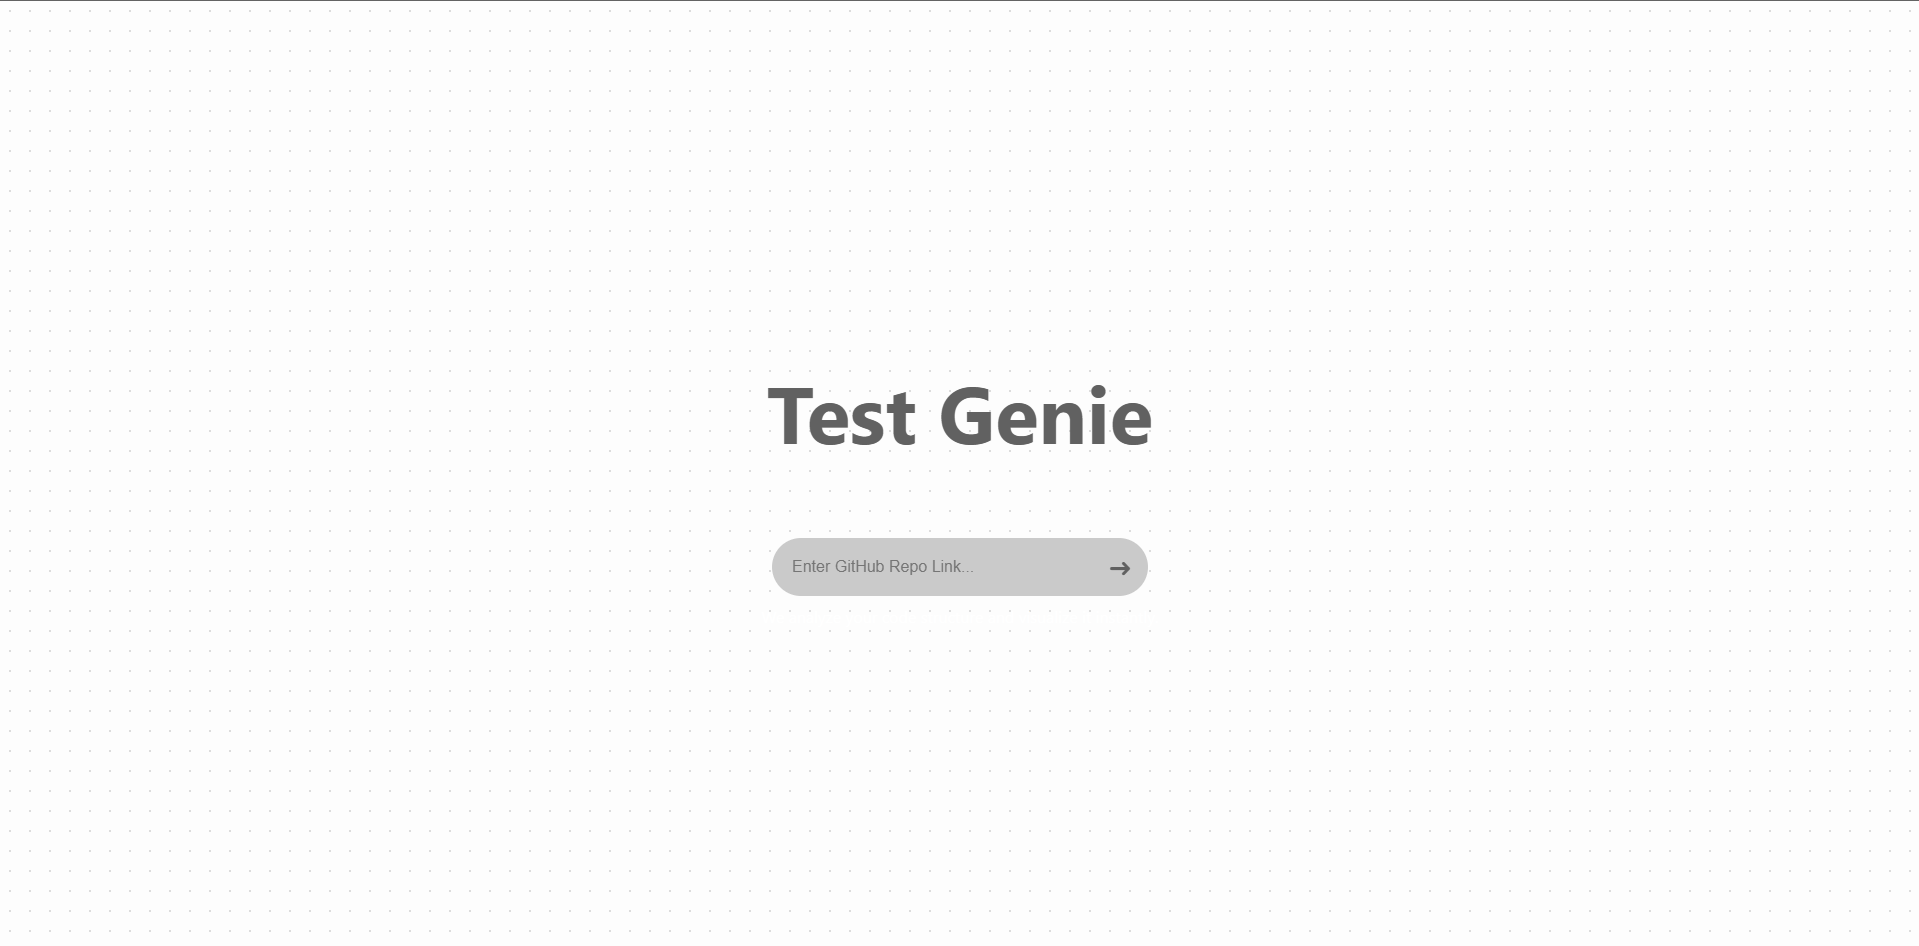
\includegraphics[width=0.8\textwidth]{images/homepage.png}
    \caption{Homepage of Test Genie system.}
    \label{fig:homepage}
\end{figure}

\subsection{Interactive Dependency Diagram}

The dependency diagram visualization represents one of the most technically challenging aspects of the frontend implementation. Initial prototypes suffered from performance issues with large projects and limited interactivity. Through iterative refinement, I developed a highly interactive visualization that balances performance with functional richness:

\begin{figure}[H] 
    \centering
    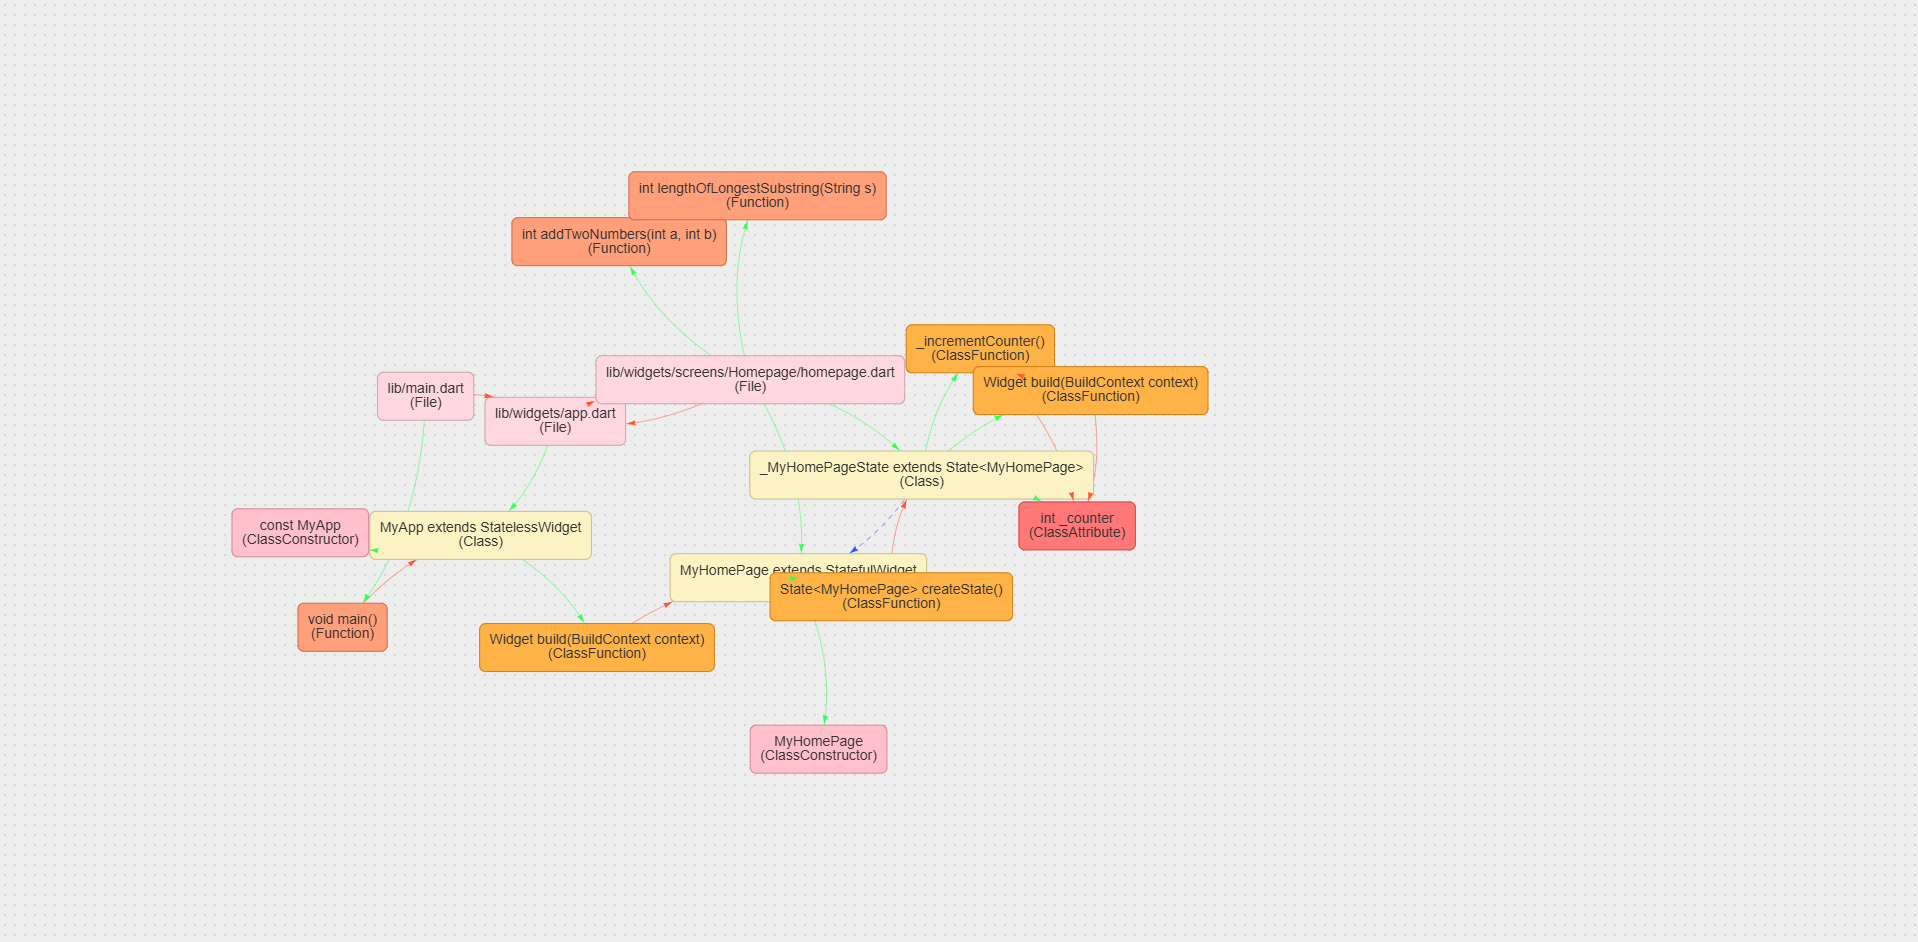
\includegraphics[width=0.8\textwidth]{images/diagram-initial_load.png}
    \caption{Initial load of the dependency diagram.}
    \label{fig:diagram-initial_load}
\end{figure}

\begin{figure}[H]
    \centering
    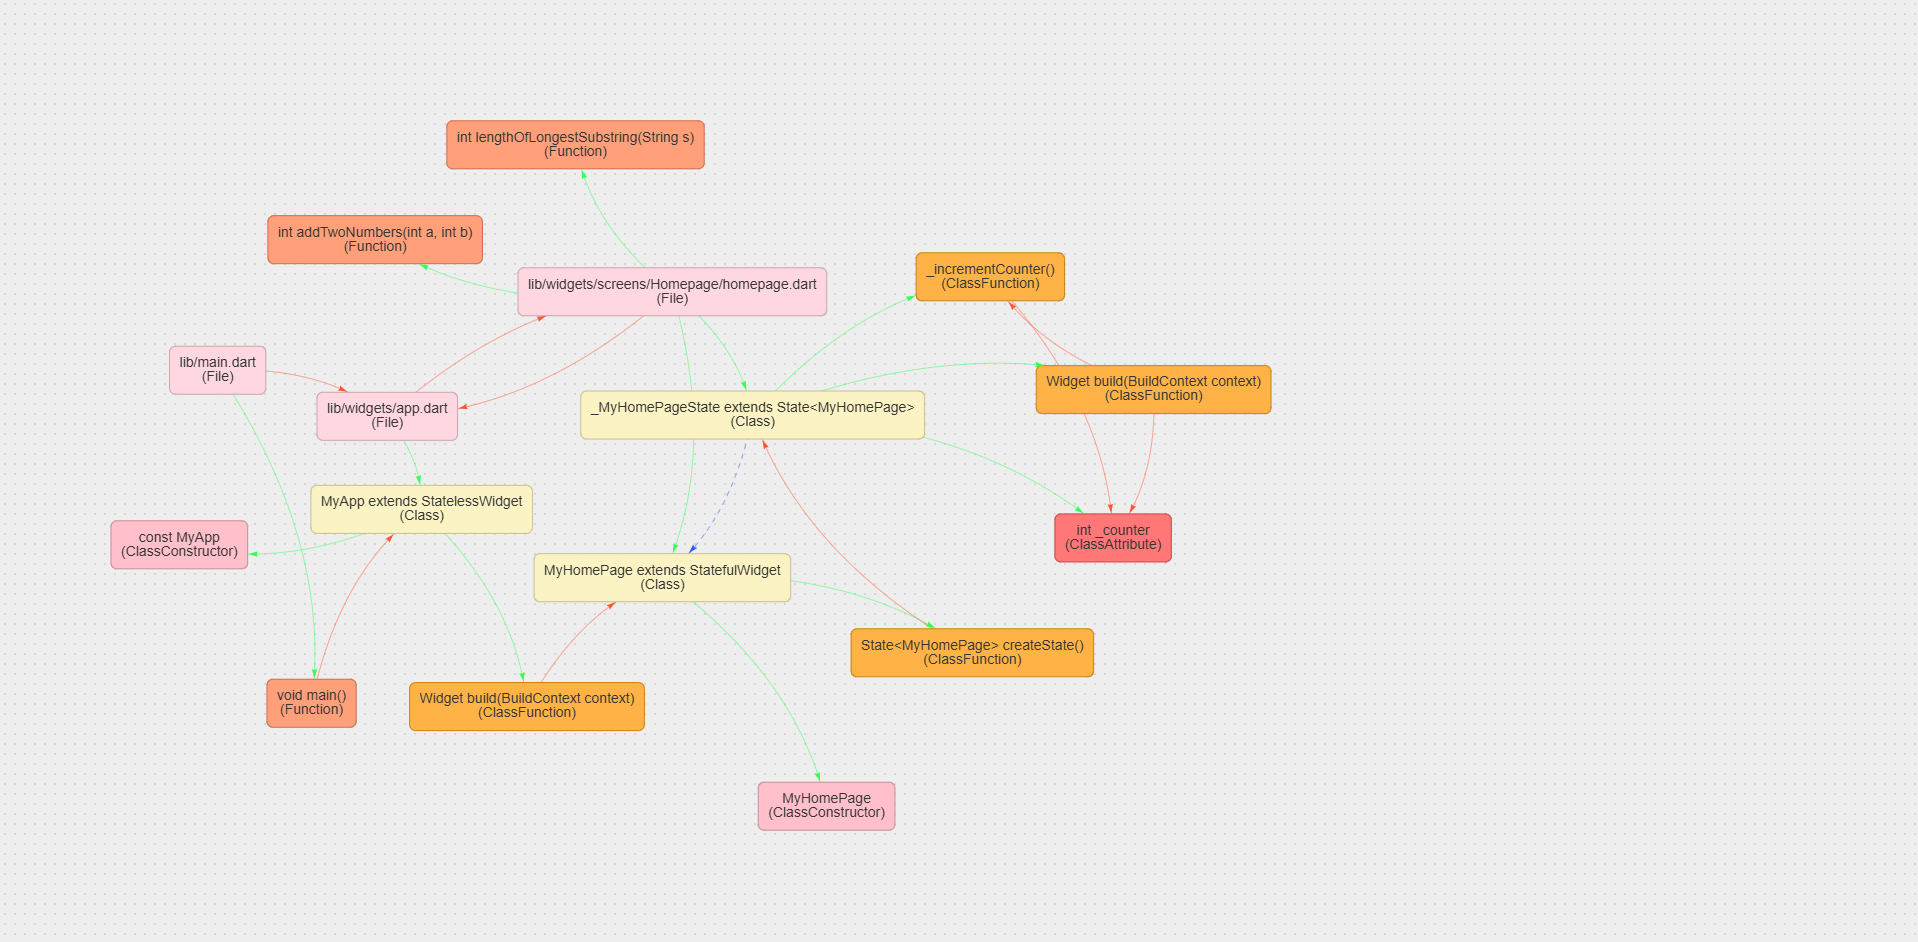
\includegraphics[width=0.8\textwidth]{images/diagram-dragged.png}
    \caption{Diagram blocks can be dragged to rearrange their positions.}
    \label{fig:diagram-dragged}
\end{figure}

The visualization incorporates several user-centric features:

\begin{itemize}
    \item \textbf{Drag and Drop}: User testing revealed the importance of manual arrangement capabilities, leading to the implementation of drag-and-drop functionality that allows users to organize the diagram according to their mental models.
    
    \item \textbf{Zoom and Pan}: To accommodate projects of varying complexity, the visualization supports intuitive zoom and pan operations that maintain context while providing detailed views of specific areas.
    
    \item \textbf{Interactive Selection}: Clickable blocks provide direct access to detailed information, establishing a natural exploration flow from overview to specific details.
\end{itemize}

\subsection{Block Detail View}

The block detail view evolved significantly based on user feedback, transitioning from a simple code display to a comprehensive information panel:

\begin{figure}[H]
    \centering
    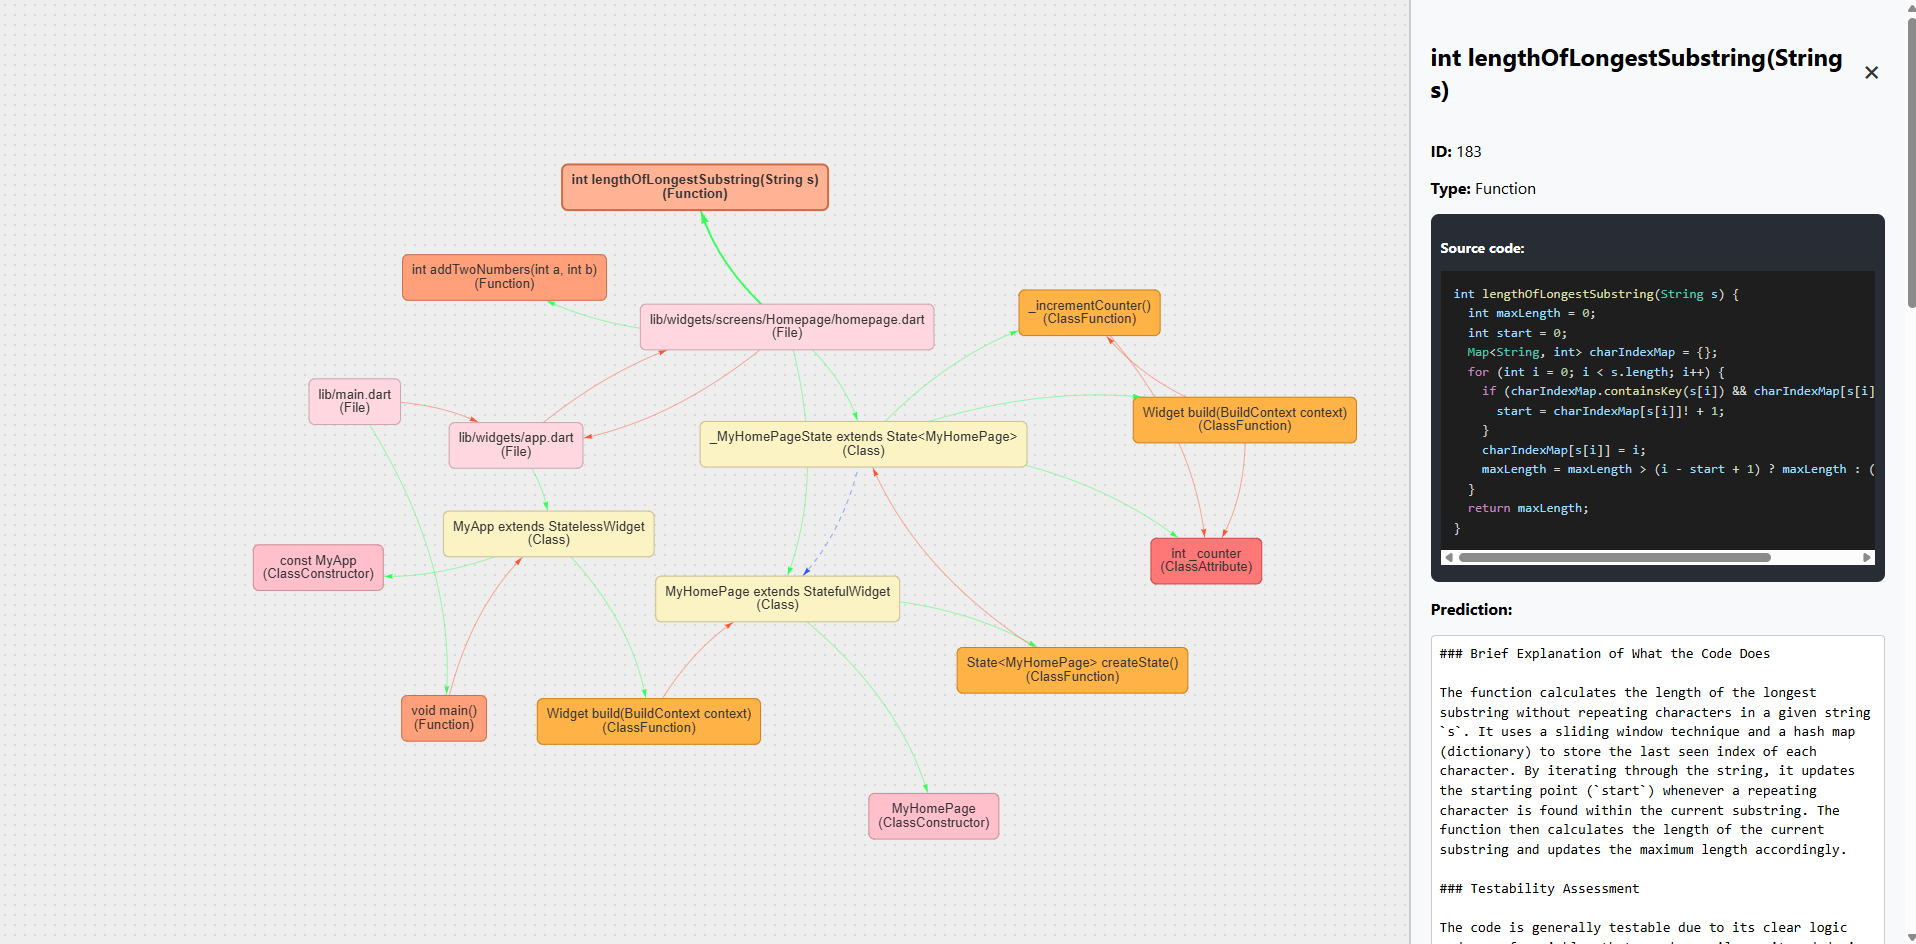
\includegraphics[width=0.8\textwidth]{images/block_detail.png}
    \caption{Block Detail View showcasing the block's content and prediction.}
    \label{fig:block-detail}
\end{figure}

Key features of this view include:

\begin{itemize}
    \item \textbf{Syntax-Highlighted Source Code}: The implementation incorporates syntax highlighting to enhance code readability, with careful attention to Dart's specific syntactic elements.
    
    \item \textbf{Prediction Display}: AI-generated predictions are presented in a structured format that emphasizes key insights while maintaining readability.
    
    \item \textbf{Editing Capabilities}: Based on the observation that AI predictions occasionally require refinement, the interface includes editing capabilities that allow users to adjust and enhance the generated insights.
    
    \item \textbf{Test Preview}: When tests have been generated, the view provides direct access to their content, creating a cohesive workflow from analysis to test review.
\end{itemize}

\subsection{Adjustable Predictions}

The prediction adjustment interface exemplifies the system's human-in-the-loop philosophy, allowing users to refine and enhance AI-generated insights based on their domain knowledge:

\begin{figure}[H]
    \centering
    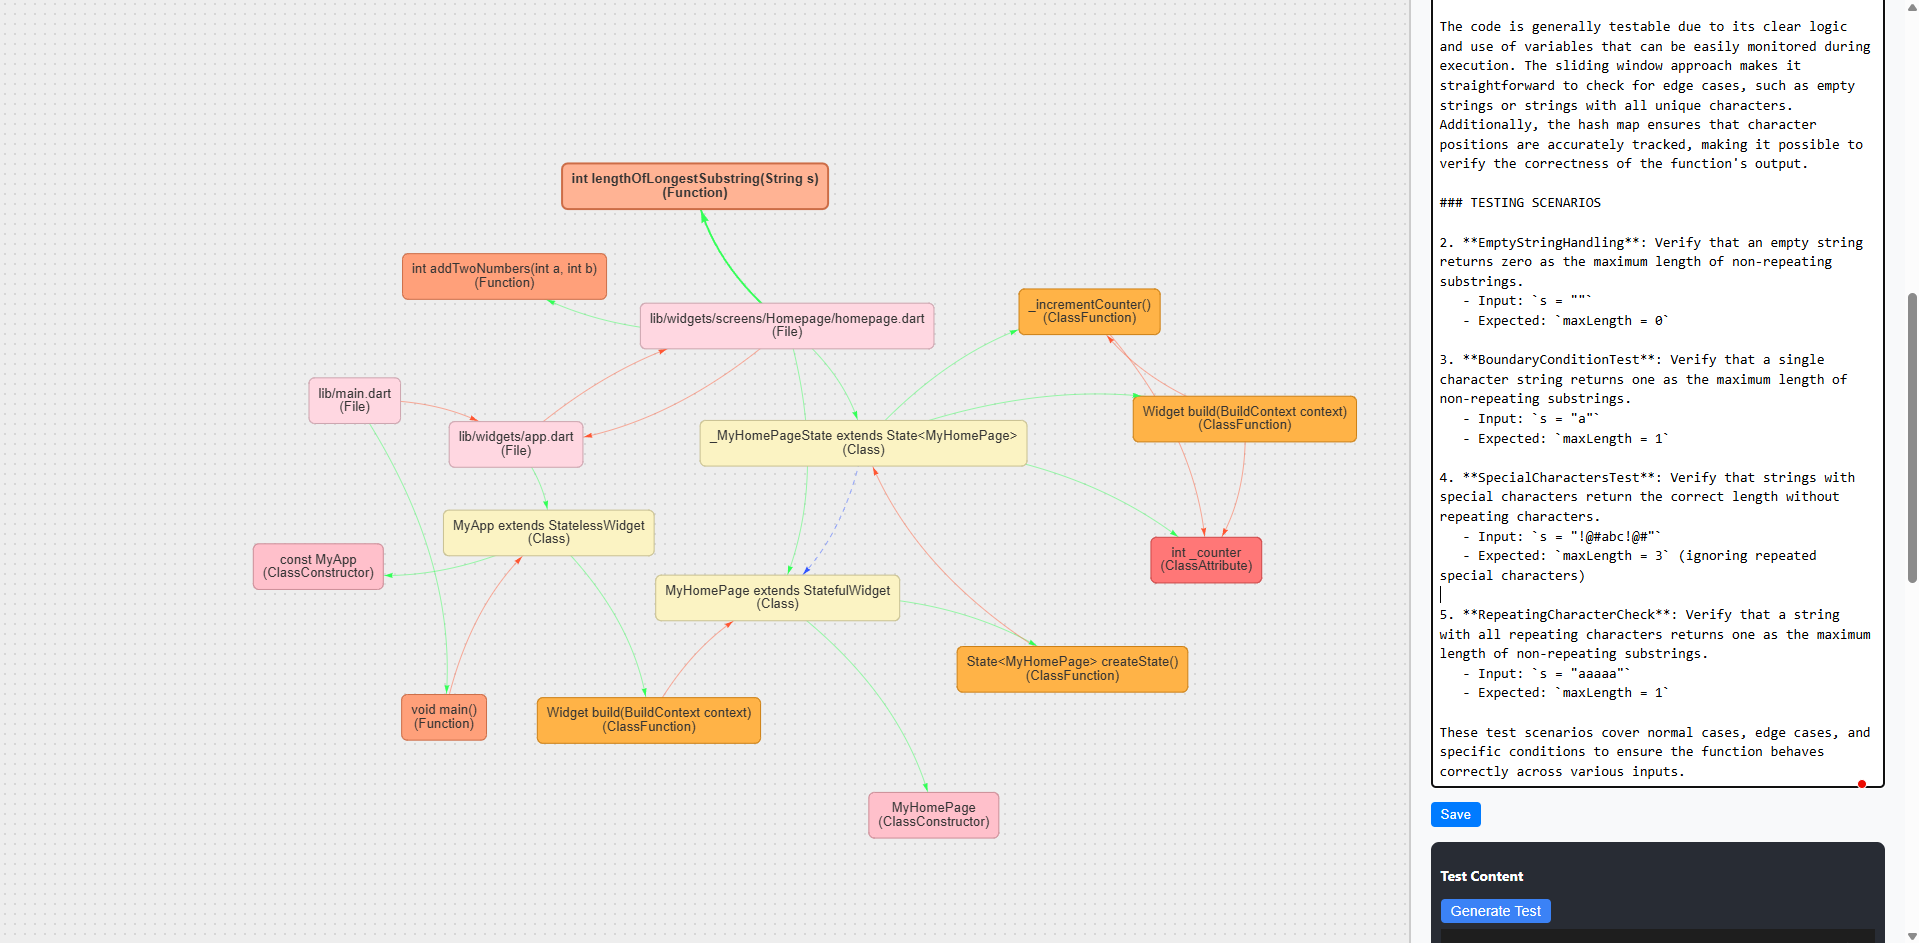
\includegraphics[width=0.8\textwidth]{images/prediction-adjustable.png}
    \caption{Prediction adjustment interface for refining AI-generated predictions.}
    \label{fig:prediction-adjustable}
\end{figure}

This feature emerged from the observation that while AI predictions are generally accurate, they occasionally benefit from human refinement, particularly for domain-specific or unusual code patterns. The interface provides direct editing capabilities with appropriate controls for saving and applying changes.

\subsection{Test Generation}

The test generation interface represents the culmination of the system's workflow, presenting users with concrete test implementations derived from the analysis process:

\begin{figure}[H]
    \centering
    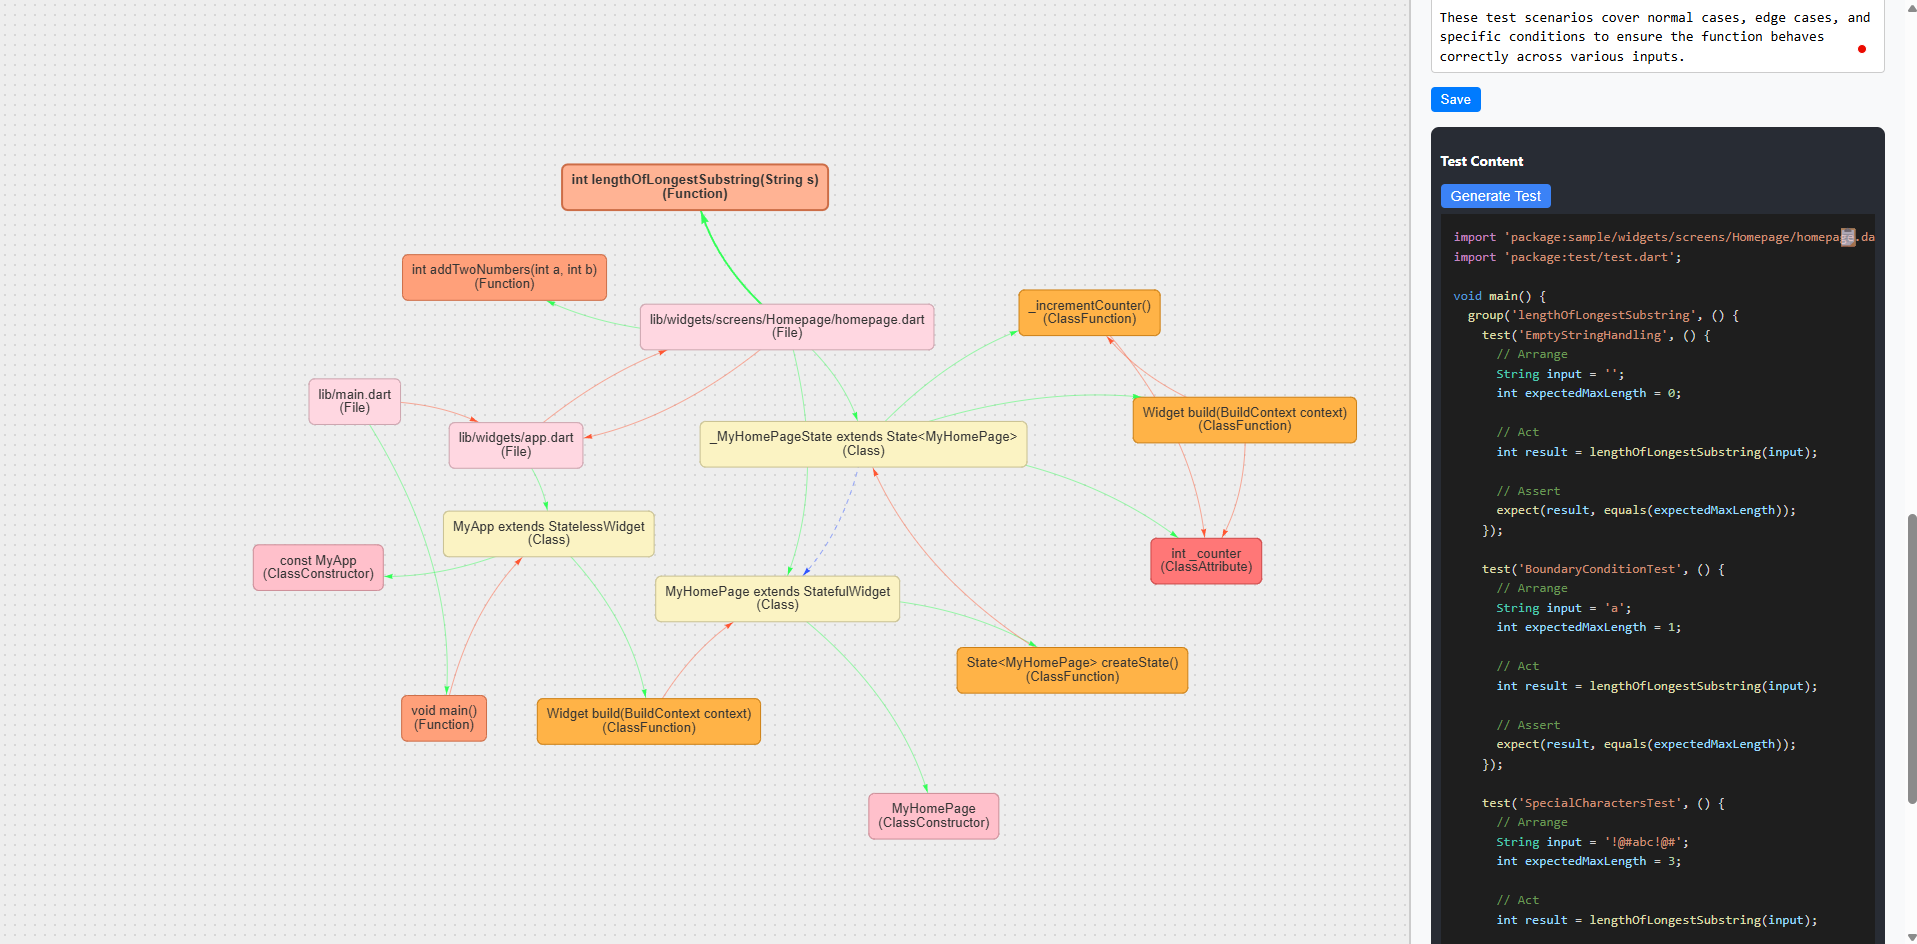
\includegraphics[width=0.8\textwidth]{images/generated_test.png}
    \caption{Generated test cases for a specific block.}
    \label{fig:generated-test}
\end{figure}

This interface incorporates several usability enhancements:

\begin{itemize}
    \item \textbf{Syntax Highlighting}: Generated tests include syntax highlighting to enhance readability and facilitate code understanding.
    
    \item \textbf{Convenient Copy Functionality}: After observing common user workflows, I added a copy button that allows users to easily transfer test code to their development environments.
    
    \item \textbf{Context Preservation}: The interface maintains the connection between the generated test and its source block, enabling users to understand the relationship between implementation and verification.
\end{itemize}

\subsection{Summary of Interactions}

The Test Genie system establishes a cohesive workflow that guides users from project initialization through analysis and test generation. Through careful attention to interaction design and component integration, the system creates a seamless experience that enhances developer productivity while maintaining visibility into the analytical and generative processes.

The visualization capabilities provide intuitive access to complex code structures, while the test generation features produce executable tests that validate code behavior. By combining visual exploration with intelligent analysis and generation, the system offers a comprehensive approach to understanding and testing Flutter applications.